\documentclass[11pt, twoside, pdftex]{article}

% This include all the settings that we should use for the document
\newcommand{\PDFTitle}{Using GDB with Nios\textsuperscript{\textregistered} V}
\newcommand{\commonPath}{../../Common}
\newcommand{\datePublished}{Mar 2022}

\newcommand{\versnum}{21.1} %version number quartus/AMP
\newcommand{\quartusname}{Quartus\textsuperscript{\textregistered} Prime}	
\newcommand{\textBar}{For \quartusname{} \versnum{}}
\newcommand{\thisyear}{2022 } %for copyright
\newcommand{\company}{FPGAcademy.org}
\newcommand{\longteamname}{FPGAcademy.org}
\newcommand{\teamname}{FPGAcademy}
\newcommand{\website}{FPGAcademy.org}

\newcommand{\productAcronym}{AMP}
\newcommand{\productNameShort}{Monitor Program}

\newcommand{\productNameMedTM}{Monitor Program}
\newcommand{\productNameMed}{Monitor Program}

%\newcommand{\headerLogoFilePath}[1]{#1/FPGAcademy.png}



\setlength\topmargin{-0.25in}
\setlength\headheight{0in}
\setlength\headsep{0.35in}
\setlength\textheight{8.5in}
\setlength\textwidth{7in}
\setlength\oddsidemargin{-0.25in}
\setlength\evensidemargin{-0.25in}
\setlength\parindent{0.25in}
\setlength\parskip{0in} 

\pdfpagewidth 8.5in
\pdfpageheight 11in

% listings is a package that supports encapsulating source code in LaTeX conveniently

\usepackage{listings}
% add support for graphics
\usepackage{graphicx}
\usepackage[usenames, dvipsnames]{color}

\def\expandparam\lstinputlisting[#1]#2{\edef\tmp{\noexpand\lstinputlisting[#1]{#2}}\tmp}

\widowpenalty 10000
\clubpenalty 10000

%%%%%%%%%%%%%%%%%%%% Source Code Formatting %%%%%%%%%%%%%%%%%%%%
\definecolor{globalCommentColour}{rgb}{0.588,0.588,0.588}

%%%%%%%%%%%%%%%%%%%%%%%%%%%%%%%%%%%%%%%%%%%%%%%%%%%%
% Defining a NiosII ASM highlighter for lstlisting
\lstdefinelanguage[NiosII]{Assembler} {
 	morekeywords={add, addi, and, andhi, andi, beq, bge, bgeu, bgt, bgtu, ble,  bleu, blt, bltu, bne, br, break,% 
 	bret, call, callr, cmpeq, cmpeqi, cmpge, cmpgei, cmpgeu, cmpgeui, cmpgt, cmpgti, cmpgtu, cmpgtui, cmple,%
 	cmplei, cmpleu, cmpleui, cmplt, cmplti, cmpltu, cmpltui, cmpne, cmpnei, custom, div, divu, eret, flushd,%
 	flushda, flushi, flushp, initd, initda, initi, jmp, jmpi, ldb, ldbio, ldbu, ldbuio, ldh, ldhio, ldhu, ldhuio,%
 	ldw, ldwio, mov, movhi, movi, movia, movui, mul, muli, mulxss, mulxsu, mulxuu, nextpc, nop, nor, or, orhi, ori,%
 	rdctl, rdprs, ret, rol, roli, ror, sll, slli, sra, srai, srl, srli, stb, stbio, sth, sthio, stw, stwio,%
 	sub, subi, sync, trap, wrctl, wrtcl, wrprs, xor, xori, xorhi, xori},% 	
 	morekeywords=[2]{.abort, .ABORT, .align, .app-file, .ascii, .asciz, .balign, .byte, .comm, .data, .def,%
 	.desc, .dim, .double, .eject, .else, .end, .endef, .endif, .equ, .equiv, .err, .extern, .file, .fill, .float,%
 	.global, .globl, .hword, .ident, .if, .include, .int, .irp, .irpc, .lcomm, .lflags, .line, .linkonce, .ln,%
 	.list, .long, .macro, .mri, .nolist, .octa, .org, .p2align, .psize, .quad, .rept, .sbttl, .scl, .section,%
 	.set, .short, .single, .size, .sleb128, .skip, .space, .stadb, .stabn, .stabs, .string, .symver, .tag,%
 	.text, .title, .type, .val, .uleb128, .word},% 	
 	morekeywords=[3]{et, bt, gp, sp, fp, ea, sstatus, ra, pc, status, estatus, bstatus, ienable, ipending, cpuid,%
 	exception, pteaddr, tlbacc, tlbmisc, eccinj, badaddr, config, mpubase, mpuacc},% 	
 	sensitive=t,%
 	alsoletter=.,%
	morestring=[b]",%
 	morecomment=[s]{/*}{*/},%
 	morecomment=[l]\#,%
   }[keywords,comments,strings]
   
   %% NOTE: morekeywords=[2] are GNU directives.
   
   \definecolor{niosInstructionColour}{rgb}{0.000,0.608,0.000}
   \definecolor{niosDirectiveColour}{rgb}{0.000,0.000,0.902}
   \definecolor{niosSpecialRegColour}{rgb}{0.000,0.000,0.000}
   \definecolor{niosStringColour}{rgb}{0.808,0.482,0.000}
   
   %% NOTE: To make bold use: =\bfseries\color{<colour>}
   \lstdefinestyle{defaultNiosStyle} {
   language=[NiosII]{Assembler},
   stringstyle=\color{niosStringColour},
   keywordstyle=\color{niosInstructionColour},
   keywordstyle=[2]\color{niosDirectiveColour},
   keywordstyle=[3]\itshape\color{niosSpecialRegColour}
   }
%%%%%%%%%%%%%%%%%%%%%%%%%%%%%%%%%%%%%%%%%%%%%%%%%%%%

%%%%%%%%%%%%%%%%%%%%%%%%%%%%%%%%%%%%%%%%%%%%%%%%%%%%
% Defining a ArmA9 ASM highlighter for lstlisting
\lstdefinelanguage[ArmA9]{Assembler} {
 	morekeywords={ADC, ADD, ADDS, AND, ANDS, B, BAL, BEQ, BGE, BGT, BL, BLT, BIC, BKPT, BLX, BNE, BX, CDP, CLZ, CMN, CMP, EOR,%
 	EORS, LDC, LDM, LDR, LDRB, LDRBT, LDRH, LDRSB, LDRSH, LDRT, LSL, MCR, MLA, MOV, MOVW, MOVT, MRC, MRS, MSR, MUL, MVN, ORR, PLD,%
 	ROR, RSB, RSC, SBC, SMLAL, SMULL, STC, STM, STR, STRB, STRBT, STRH, STRT, SUB, SUBS, SWI, SWP, SWPB, TEQ, UMLAL,
 	PUSH, POP, MOVS, RORS, LSR},%
 	morekeywords=[2]{.abort, .ABORT, .align, .app-file, .ascii, .asciz, .balign, .byte, .comm, .data, .def,%
 	.desc, .dim, .double, .eject, .else, .end, .endef, .endif, .equ, .equiv, .err, .extern, .file, .fill, .float,%
 	.global, .globl, .hword, .ident, .if, .include, .int, .irp, .irpc, .lcomm, .lflags, .line, .linkonce, .ln,%
 	.list, .long, .macro, .mri, .nolist, .octa, .org, .p2align, .psize, .quad, .rept, .sbttl, .scl, .section,%
 	.set, .short, .single, .size, .sleb128, .skip, .space, .stadb, .stabn, .stabs, .string, .symver, .tag,%
 	.text, .title, .type, .val, .vectors, .uleb128, .word},%
 	morekeywords=[3]{SP, PC, MIDR, CTR, TCMTR, TLBTR, MPIDR, ID_PFR0, ID_PFR1, ID_DFR0, ID_MMFR0, ID_MMFR1, ID_MMFR2,%
 	ID_MMFR3, ID_ISAR0, ID_ISAR1, ID_ISAR2, ID_ISAR3, ID_ISAR4, CCSIDR, CLIDR, AIDR, CSSELR, TTBR0, TTRB1, TTBR2, DACR,%
 	DFSR, IFSR, ADFSR, AIFSR, DFAAR, IFAR, ICIALLUIS, BPIALLIS, PAR, ICIALLU, ICIMVAU, BPIALL, DCIMVAC, DCISW, V2PCWPR,%
 	DCCVAC, DCCSW, DDIMVAC, DCISW, TLBALLIS, TLBIMVAIS, TLBIASIDIS, TLBIMVAAIS, TLBIALL, TLBIMVA, TLBIASID, TLBIMVAA,%
 	PMCR, PMCNTENSET, PMCNTENCLR, PMOVSR, PMSWINC, PMSELR, PMXEVTYPER, PMXEVCNTR, PMUSERENR, PMINTENSET, PMINTENCLR,%
 	PRRR, NRRR, PLEIDR, PLEASR, PLEFSR, PLEUAR, PLEPCR, VBAR, MVBAR, ISR, FCSEIDR, CONTEXTIDR, TPIDRURW, TPIDRURO, TPIDRPRW},%
 	sensitive=f,%
 	alsoletter=.,%
	morestring=[b]",%
 	morecomment=[s]{/*}{*/},%
 	morecomment=[l]{//},%
   }[keywords,comments,strings]
   
   %% NOTE: morekeywords=[2] are GNU directives.
   
   \definecolor{armInstructionColour}{rgb}{0.000,0.608,0.000}
   \definecolor{armDirectiveColour}{rgb}{0.000,0.000,0.902}
   \definecolor{armSpecialRegColour}{rgb}{0.000,0.000,0.000}
   \definecolor{armStringColour}{rgb}{0.808,0.482,0.000}
   
   \lstdefinestyle{defaultArmStyle} {
   language=[ArmA9]{Assembler},
   stringstyle=\color{armStringColour},
   keywordstyle=\color{armInstructionColour},
   keywordstyle=[2]\color{armDirectiveColour},
   keywordstyle=[3]\itshape\color{armSpecialRegColour}
   }
%%%%%%%%%%%%%%%%%%%%%%%%%%%%%%%%%%%%%%%%%%%%%%%%%%%%

%%%%%%%%%%%%%%%%%%%%%%%%%%%%%%%%%%%%%%%%%%%%%%%%%%%%
% Defining style for the verilog.

\definecolor{verilogCommentColour}{rgb}{0.000,0.502,0.000}

\lstdefinestyle{defaultVerilogStyle} {
language={Verilog},
keywordstyle=\color{blue},
commentstyle=\color{verilogCommentColour}
}
%%%%%%%%%%%%%%%%%%%%%%%%%%%%%%%%%%%%%%%%%%%%%%%%%%%%

%%%%%%%%%%%%%%%%%%%%%%%%%%%%%%%%%%%%%%%%%%%%%%%%%%%%
% Defining style for the vhdl.
\lstdefinestyle{defaultVHDLStyle} {
language={VHDL},
keywordstyle=\color{blue},
commentstyle=\color{verilogCommentColour}
}
%%%%%%%%%%%%%%%%%%%%%%%%%%%%%%%%%%%%%%%%%%%%%%%%%%%%

%%%%%%%%%%%%%%%%%%%%%%%%%%%%%%%%%%%%%%%%%%%%%%%%%%%%
% Java
\definecolor{javaStringColour}{rgb}{0.808,0.482,0}
%%%%%%%%%%%%%%%%%%%%%%%%%%%%%%%%%%%%%%%%%%%%%%%%%%%%

%%%%%%%%%%%%%%%%%%%%%%%%%%%%%%%%%%%%%%%%%%%%%%%%%%%%
% Defining language styles
% C
\definecolor{CStringColour}{rgb}{0.808,0.482,0}
%%%%%%%%%%%%%%%%%%%%%%%%%%%%%%%%%%%%%%%%%%%%%%%%%%%%

%%%%%%%%%%%%%%%%%%%%%%%%%%%%%%%%%%%%%%%%%%%%%%%%%%%%
% Defining extended LaTeX language.
\lstdefinelanguage[LocalLaTeX]{TeX}[LaTeX]{TeX}%
 	{moretexcs={bf, it, sf, lstset},%
   	}%

\lstdefinestyle{defaultLocalLatexStyle} {
language=[LocalLatex]{TeX},
keywordstyle=\color{blue}\bfseries,
keywordstyle=[2]\color{blue},
keywordstyle=[3]\color{blue}\bfseries
}
%%%%%%%%%%%%%%%%%%%%%%%%%%%%%%%%%%%%%%%%%%%%%%%%%%%%

\lstset{
%language = C,
%language = Verilog,
%basicstyle=\color{black}\rmfamily\ttfamily,
basicstyle=\small\color{black}\ttfamily,
commentstyle=\small\color{globalCommentColour}\itshape\ttfamily,
keywordstyle=\small\color{blue}\bfseries\ttfamily,
showstringspaces=false,
frame=none, %lines % boxed listings
breaklines=true,
breakatwhitespace=true,
tabsize=4
}
%%%%%%%%%%%%%%%%%%%%%%%%%%%%%%%%%%%%%%%%%%%%%%%%%%%%%%%%%%%%%%%%


%\usepackage[centering]{geometry}.
%%%%%%%%%%%%%%%%%%%%%%%%%%%%%%%%%%%%%%%%%%%%%%%%%%%
% Document Settings
\usepackage[labelsep=period]{caption}
% we can choose a better font later
%\usepackage{palatino}
\usepackage{fourier}
%\fontencoding{T1}
% include common used symbols
\usepackage{textcomp}
% add support for graphics
\usepackage{graphicx}
\usepackage[usenames, dvipsnames]{color}
% enable to draw thick or thin table hlines
\setlength{\doublerulesep}{\arrayrulewidth}
\usepackage{longtable}
\setlongtables
%\usepackage{array}
% It may be better to use PDFLaTeX as it can generate bookmarks for the
% document

% Add some useful packages
\usepackage{ae,aecompl}
\usepackage{epsfig,float,times}

% reset the font for section
\usepackage{sectsty}
%\allsectionsfont{\fontfamily{ptm}\selectfont}
\allsectionsfont{\usefont{OT1}{phv}{bc}{n}\selectfont}

% use compact space for sections
\usepackage[compact]{titlesec}
\titlespacing{\section}{0pt}{0.2in}{*0}
\titlespacing{\subsection}{0pt}{0.1in}{*0}
\titlespacing{\subsubsection}{0pt}{0.05in}{*0}

% fancyhdr header and footer customization
\usepackage{layout}
\usepackage{fancyhdr}
\pagestyle{fancy}
\fancyhead{}
\fancyhead[R]{\textit{\tiny{\textBar}}}
\fancyfoot{}
\fancyfoot[LO,
RE]{\textrm{\href{https://www.fpgacademy.org}{\small \longteamname}} \\ {\small \datePublished }}
\fancyfoot[RO, LE]{\small \thepage}
% two-side settings
%\fancyhead{} % clear all header fields
%\fancyfoot{} % clear all footer fields
%\fancyfoot[LE,RO]{\thepage}
\renewcommand{\headrulewidth}{2pt}
\renewcommand{\headrule}{{\color{blue} \hrule width\headwidth height\headrulewidth \vskip-\headrulewidth}}
\renewcommand{\footrulewidth}{0pt}

% Format the footer on page 1
\fancypagestyle{plain}{
\fancyhead{}
\fancyfoot{}
\fancyfoot[LO,
RE]{\textrm{\href{https://www.fpgacademy.org}{\small \longteamname}} \\ {\small \datePublished }}
\fancyfoot[RO, LE]{\small \thepage}
\renewcommand{\headrulewidth}{0pt}
}
% adjust some setting to try to make the figure stay in the same page with text
% Reference: 	http://www.cs.uu.nl/~piet/floats/node1.html
%   			http://mintaka.sdsu.edu/GF/bibliog/latex/floats.html
%   General parameters, for ALL pages:
\renewcommand{\topfraction}{0.9}	% max fraction of floats at top
\renewcommand{\bottomfraction}{0.8}	% max fraction of floats at bottom
%   Parameters for TEXT pages (not float pages):
\setcounter{topnumber}{3}
\setcounter{bottomnumber}{3}
\setcounter{totalnumber}{5}     % 2 may work better
\setcounter{dbltopnumber}{2}    % for 2-column pages
\renewcommand{\dbltopfraction}{0.9}	% fit big float above 2-col. text
\renewcommand{\textfraction}{0.07}	% allow minimal text w. figs
%   Parameters for FLOAT pages (not text pages):
\renewcommand{\floatpagefraction}{0.7}	% require fuller float pages
% N.B.: floatpagefraction MUST be less than topfraction !!
\renewcommand{\dblfloatpagefraction}{0.7}	% require fuller float pages
%%%%%%%%%%%%%%%%%%%%%%%%%%%%%%%%%%%%%%%%%%%%%%%%%%%
% remember to use [htp] or [htpb] for placement
%%%%%%%%%%%%%%%%%%%%%%%%%%%%%%%%%%%%%%%%%%%%%%%%%%%

% set no indent for paragraph
\setlength{\parindent}{0em}
\addtolength{\parskip}{11pt}
\newcommand{\compact}{[topsep=0pt]}
% use this package to reduce space
\usepackage{enumitem}
\usepackage{multirow}
\usepackage{rotating}
\usepackage{pifont}
\usepackage{dingbat}
\newcommand{\itemsecond}{$\circ$}
%
%%%%%%%%%%%%%%%%%%
\date{}
\author{}
%%%%%%%%%%%%%%%%%%
\newcommand{\de}{DE-series}
\newcommand{\up}{FPGAcademy}
\newcommand{\fabric}{Avalon Switch Fabric}
\newcommand{\TODO}[1]{\textcolor{red}{\textbf{TODO}: #1}}
\def\registered{{\ooalign{\hfil\raise .00ex\hbox{\scriptsize R}\hfil\crcr\mathhexbox20D}}}

% enable url and reference(bookmarks) in pdf
\usepackage{url}
\usepackage[pdftex, colorlinks]{hyperref}
\hypersetup{%
pdftitle={\PDFTitle},
linkcolor=blue,
hyperindex=true,
pdfauthor={\longteamname},
pdfkeywords={FPGAcademy, Academic Program, Example System},
bookmarksnumbered,
bookmarksopen=false,
filecolor=blue,
pdfstartview={FitH},
urlcolor=blue,
plainpages=false,
pdfpagelabels=true,
linkbordercolor={1 1 1} %no color for link border
}%
%%%%%%%%%%%%%%%%%%%%%%%%%%%%%%%%%%%%%%%%%%%%%%%%%%%
\setlength{\fboxsep}{0.7pt}
\setlength{\fboxrule}{0.5pt}

\newcommand{\red}[1]{{\color{red}\sf{#1}}}
\newcommand{\blue}[1]{{\color{blue}\sf{#1}}}



%%%%%%%%%%%%%%%%%%%%%%%%%
% Add title
\newcommand{\doctitle}{Using GDB with Nios\textsuperscript{\textregistered} V}
\newcommand{\dochead}{Using GDB with Nios\textsuperscript{\textregistered} V}
% Usually no need to change these two lines
\title{\fontfamily{phv}\selectfont{\doctitle} }
\chead{ \small{\textsc{\bfseries \dochead} } }
% Customizations
\newenvironment{ctabbing}%
{\begin{center}\begin{minipage}{\textwidth}\begin{tabbing}}
{\end{tabbing}\end{minipage}\end{center}}

%%%%%%%%%%%%%%%%%%%%%%%%%
% Allows multiple figures per page

\renewcommand\floatpagefraction{.9}
\renewcommand\topfraction{.9}
\renewcommand\bottomfraction{.9}
\renewcommand\textfraction{.1}   
\setcounter{totalnumber}{50}
\setcounter{topnumber}{50}
\setcounter{bottomnumber}{50}
\raggedbottom

%%%%%%%%%%%%%%%%%%
%%% DOCUMENT START
%\begin{document}
\begin{document}
\begin{table}
    \centering
    \begin{tabular}{p{5cm}p{4cm}}
        \hspace{-3cm}
        &
        \raisebox{1\height}{\parbox[h]{0.5\textwidth}{\Large\fontfamily{phv}\selectfont{\textsf{\doctitle}}}}
    \end{tabular}
    \label{tab:logo}
\end{table}

\colorbox[rgb]{0,0.384,0.816}{\parbox[h]{\textwidth}{\color{white}\textsf{\textit{\textBar}}}}

\thispagestyle{plain}
 
\section{Introduction}

This tutorial provides instructions for using the {\it GNU Project Debugger} (GDB) with the 
{\it Nios}\textsuperscript{\textregistered} {\it V} processor, to 
develop and debug software programs that are written in assembly-language or C code. 

This document is intended for a reader who is using a computer system with Nios~V on one of 
the DE-series boards that are described in the \texttt{Teaching and Projects Boards} 
section of the {\small \href{https://www.fpgacademy.org/boards.html} {FPGAcademy.org}} website.
We also assume that the reader is using a computer running a recent version of the 
{\it Windows}\textsuperscript{\textregistered} Operating system.

{\bf Required Software and Hardware}:
\begin{itemize}
\item Quartus Prime Programmer
\item GDB Server and Client for Nios~V
\item Nios~V computer system and DE-series FPGA board
\item Nios~V software development tools
\end{itemize}

{\bf Contents}:
\begin{itemize}
\item Installing the required software and hardware
\item Setting up the Nios~V development environment
\item Developing and debugging Nios~V assembly-language programs
\item Developing and debugging C programs
\item GDB command reference
\end{itemize}
\clearpage
\newpage

\section{Installing the Required Software and Hardware}
\label{sec:getthem}

The main software tools that are needed for this tutorial are the FPGA {\it Programmer
Tools} that accompany the Quartus Prime CAD system, the GDB server and client for Nios~V, and 
various Nios~V software development tools. The required hardware is a Nios~V computer
system that can be programmed into a DE-series FPGA board. The procedures for downloading and 
installing each of these components on your own computer are described below. A reader who 
is using a computer that already has the required software and hardware can skip ahead to 
Section~\ref{sec:setup}. 

\subsection{Installing the Quartus Prime Programmer Tools}
\label{sec:programmer}

The Nios~V processor is implemented as part of a computer system in an Altera FPGA device. 
In this tutorial we assume that the reader is using the {\it DE1-SoC Computer with Nios~V}.
A complete description of this system, describing all of the peripherals that are
connected to Nios~V, is available as part of the \texttt{Computer Organization} course 
on {\small \href{https://www.fpgacademy.org/courses.html} {FPGAcademy.org}}. If a
different computer system is being used, then some features of the hardware may not match
those described in this tutorial.

We assume that the user has access to a {\it DE1-SoC} board, and that this board has {\it not} 
already been programmed with the {\it DE1-SoC Computer with Nios~V}. Hence, programming of 
the board has to be performed, by using the {\it Quartus Prime Programmer} tools. This 
software can be obtained from the {\it Internet}, as discussed below. 

Three different Quartus Prime software {\it packages} are available, called {\it Pro},
{\it Standard}, and {\it Lite}. For each of these packages a number of {\it versions} are
released over time.  For any Quartus package, the {\it Programmer} tools can be 
obtained as a separate, {\it stand-alone}, program or as a part of a complete 
Quartus system. When used as a stand-alone program, the {\it Programmer} tools do not 
not require any license and are free to use. But if a complete Quartus Prime system 
were to be obtained and installed, then the {\it Pro} and {\it Standard} versions would 
require paid licenses, and only the {\it Lite} version could be used without a license. For 
this tutorial we use the {\it Programmer} as a stand-alone program. Perform the following
steps to download and install this program:

\begin{enumerate}
\item Search on the {\it Internet} for the \texttt{Intel (Altera) FPGA Software Download Center}. 
\item As illustrated in Figure~\ref{fig:down1}, select a \texttt{Software Package} and 
\texttt{Version}. For this tutorial we have selected \texttt{Quartus Prime Pro} and
\texttt{Version 24.1}.
\item Scroll down on the web page to see the types of \texttt{Downloads} that are
available. Click on the \texttt{Additional Software} category. Then, scroll further down 
on the web page to reveal the \texttt{Stand-Alone Software} programs. As illustrated in
Figure~\ref{fig:down2}, click on the button that is displayed to \texttt{Download} 
the \texttt{Quartus Prime Programmer and Tools}. You will need to accept an \texttt{Agreement},
after which a file will be downloaded to your computer.

The file downloaded above is an executable program (.{\it exe}).
Open the folder on your computer where this executable file has 
been downloaded and run the program. This action opens the installer dialogue depicted in 
Figure~\ref{fig:exe1}. Click \texttt{Next} to see the license agreement, which
must be accepted to install the software. Clicking \texttt{Next} again allows you to
select an installation folder. We recommend that you accept the default location which
should be similar to the one shown in Figure~\ref{fig:exe2}. Select \texttt{Next} to advance 
to the summary screen of the installation dialogue. On this screen you may see a message about 
obtaining a license to use the software, but {\bf do not} click on the provided link, because 
no license is required for the stand-alone {\it Programmer Tools}. Click \texttt{Next} on the
summary screen to install the {\it Programmer Tools}.

\begin{figure}[H]
    \begin{center}
        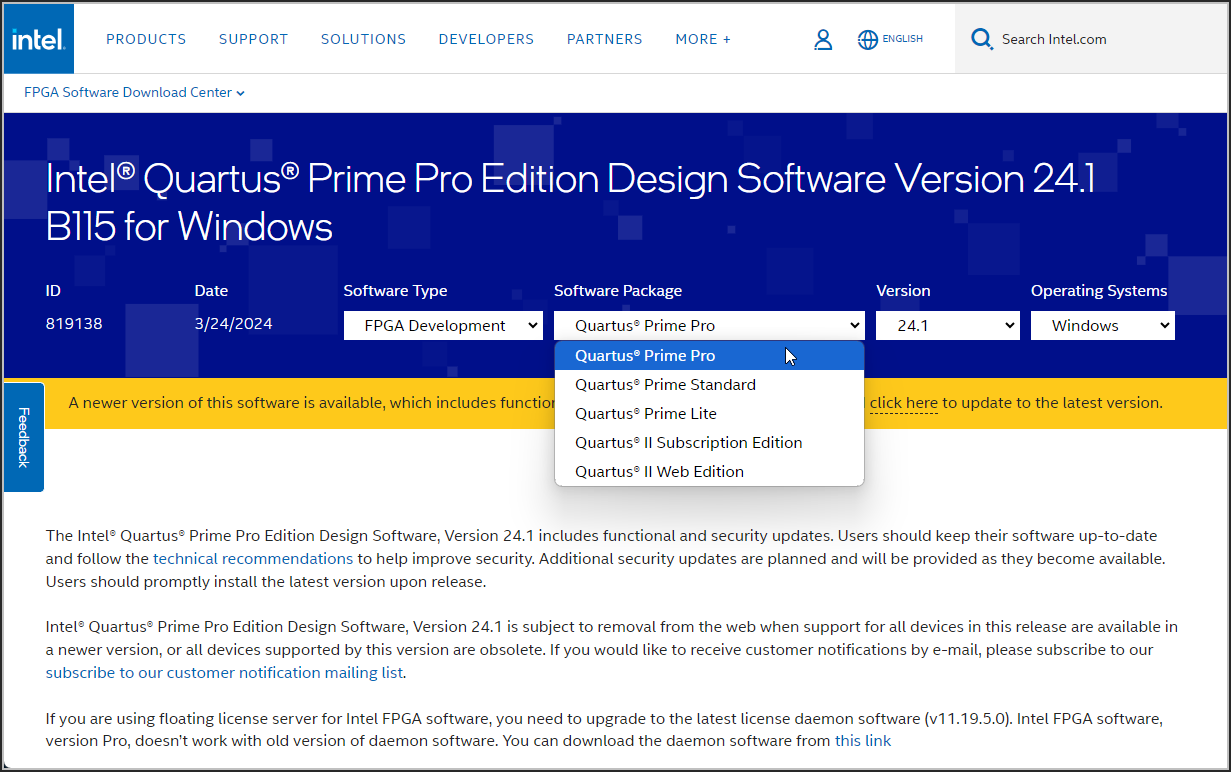
\includegraphics[width=.9\linewidth]{figures/down1.png}
        \caption{The Intel (Altera) FPGA Software Download Center.}
        \label{fig:down1}
    \end{center}
\end{figure}

\begin{figure}[H]
    \begin{center}
        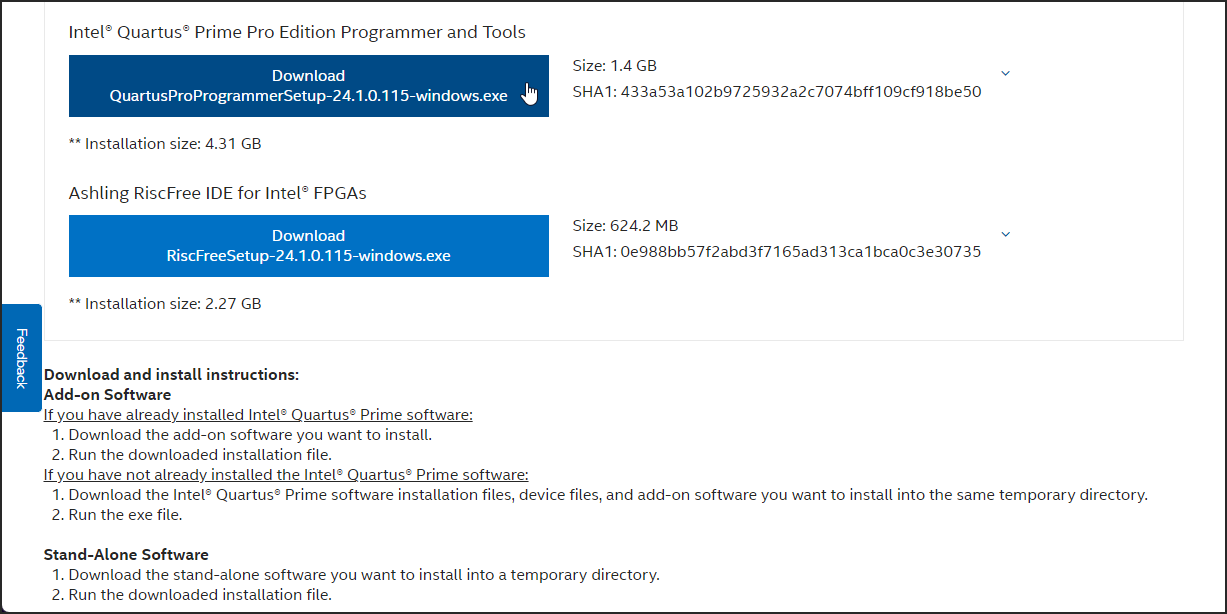
\includegraphics[width=.9\linewidth]{figures/down2.png}
        \caption{Downloading the Quartus Prime Programmer.}
        \label{fig:down2}
    \end{center}
\end{figure}

\begin{figure}[h]
    \begin{center}
        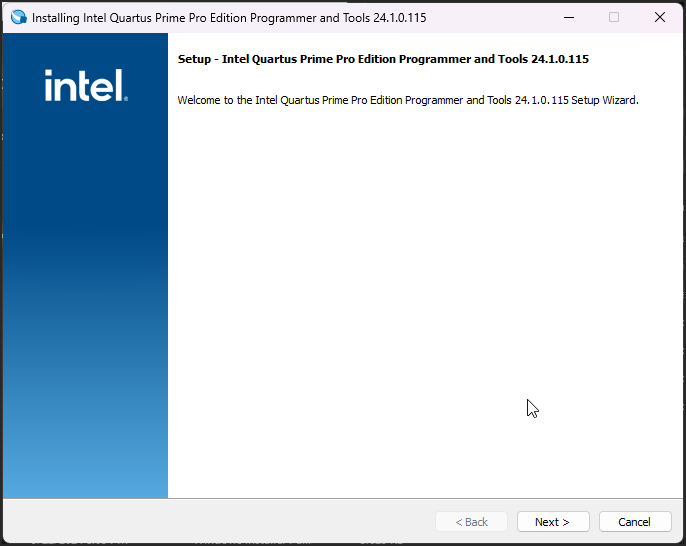
\includegraphics[scale=0.66]{figures/exe1.png}
        \caption{The {\it Programmer Tools} installation dialogue.}
        \label{fig:exe1}
    \end{center}
\end{figure}

\begin{figure}[h]
    \begin{center}
        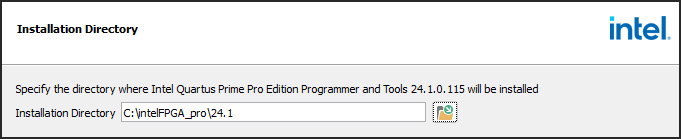
\includegraphics[scale=0.66]{figures/exe2.png}
        \caption{Choosing the installation folder.}
        \label{fig:exe2}
    \end{center}
\end{figure}

\begin{figure}[h]
    \begin{center}
        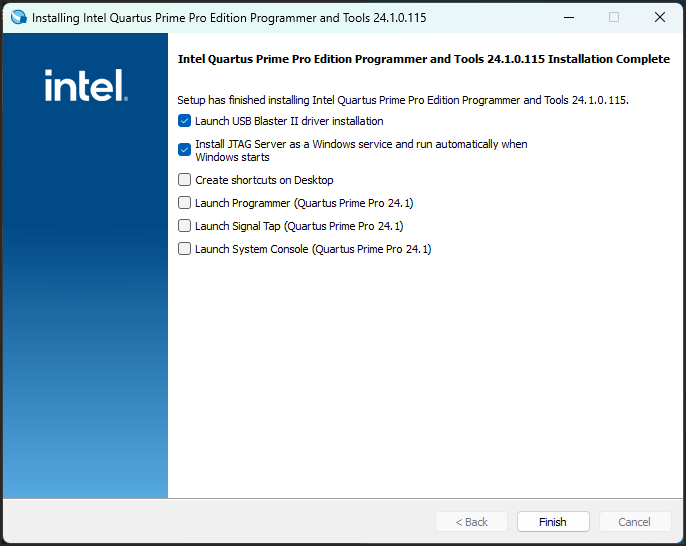
\includegraphics[scale=0.66]{figures/down2a.png}
        \caption{Post-installation selections.}
        \label{fig:down2a}
    \end{center}
\end{figure}

\item
After completing the {\it Programmer Tools} installation, the window displayed in 
Figure~\ref{fig:down2a} may appear. As the figure indicates you should make the
selections for installing the \texttt{USB Blaster II} driver and the \texttt{JTAG Server}. 
Click {\it Finish}. Depending on what device drivers are already installed on your computer 
you may be presented with additional installation dialogues. If so, follow the presented
steps to install the necessary drivers. These drivers allow for communication between your
computer and an FPGA board that is connected to the computer via a USB cable. 
\end{enumerate}

\newpage
\subsection{Installing the GDB Server and Client for Nios~V}
\label{sec:gdb}

The GDB software tools for Nios~V that are needed for this tutorial are available from the same 
\texttt{Intel (Altera) FPGA Software Download Center} used above to obtain the 
Quartus {\it Programmer Tools}. Navigate again to the website that is depicted in
Figure~\ref{fig:down1}. Again, scroll down on the website to see the types of
\texttt{Downloads} that are available, click on the \texttt{Additional Software} category,
and scroll further down to display the \texttt{Stand-Alone Software} programs. The 
GDB software tools for Nios~V are part of the package called 
\texttt{Ashling RiscFree IDE for Intel FPGAs}.
Click to download this package as indicated in Figure~\ref{fig:down3}, after which a file
will be downloaded to your computer.

The file downloaded above is an executable program (.{\it exe}).  Open the folder 
on your computer where this executable file has been downloaded and run the program.
This action opens the installer dialogue depicted in Figure~\ref{fig:exe3}. 
Click \texttt{Next} to see the license agreement, which
must be accepted to install the software. Clicking \texttt{Next} again allows you to
select an installation folder. This folder must be the {\it same} as the one that you
selected for the Quartus Programmer Tools, as mentioned previously for 
Figure~\ref{fig:exe2}. Select \texttt{Next} 
to advance to the summary screen of the installation dialogue. On this screen you may see a 
message about obtaining a license to use the software, but {\bf do not} click on the 
provided link, because no license is required for the this software package. After the
software has been installed, click \texttt{Finish} to close the installation executable.

\begin{figure}[H]
    \begin{center}
        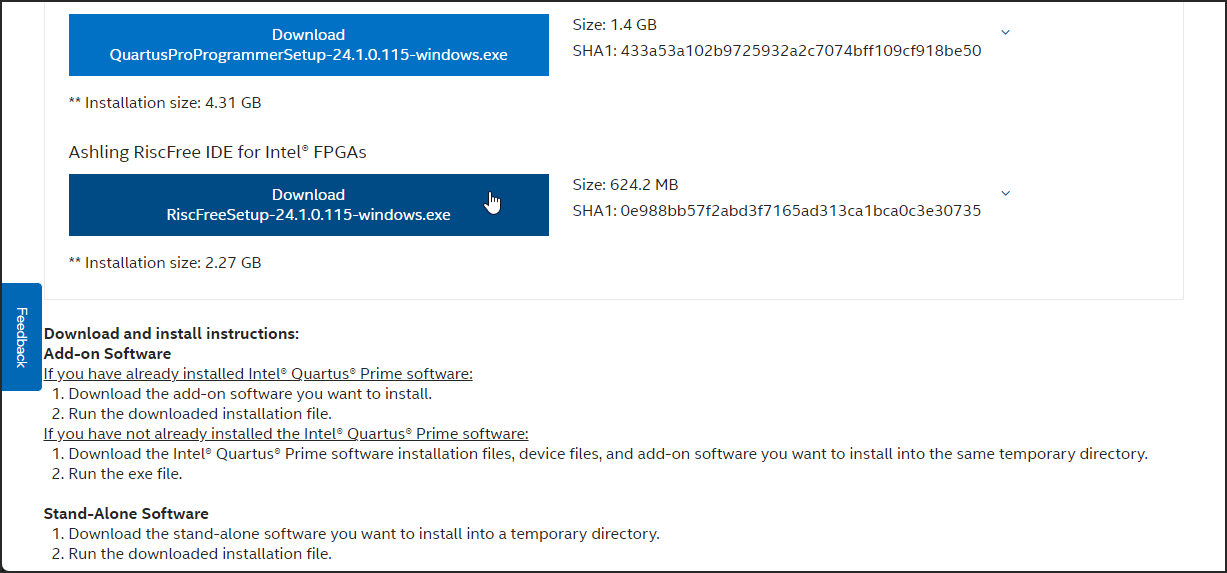
\includegraphics[width=.9\linewidth]{figures/down3.png}
        \caption{Downloading the GDB tools.}
        \label{fig:down3}
    \end{center}
\end{figure}

\begin{figure}[h]
    \begin{center}
        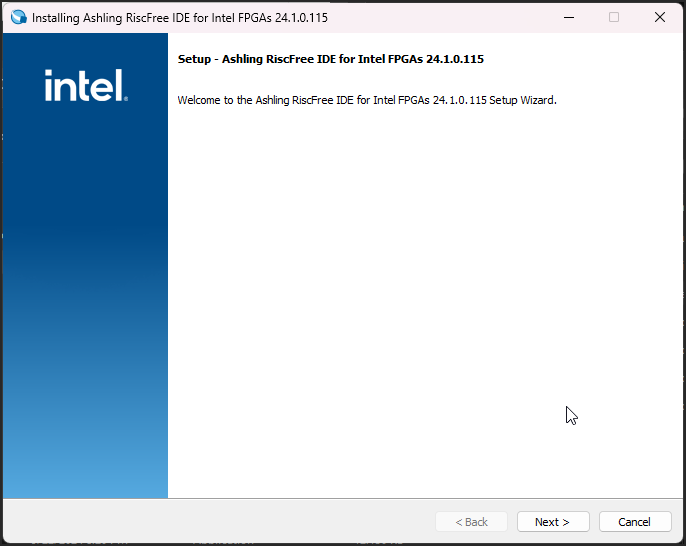
\includegraphics[scale=0.66]{figures/exe3.png}
        \caption{The {\it Ashling RiscFree Software} installation dialogue.}
        \label{fig:exe3}
    \end{center}
\end{figure}

\subsection{Installing the Nios~V Hardware and Software Development Tools}
\label{sec:hw_sw}

This tutorial requires a hardware system containing the Nios~V processor, as well as Nios~V
software development tools for that system. These hardware and software components can be
obtained from {\it GitHub}, at the \texttt{URL} below:

{\href{https://github.com/fpgacademy/beta\_releases/releases/tag/beta0.2} 
{https://github.com/fpgacademy/beta\_releases/releases/tag/beta0.2}.

From the GitHub repository download to your computer the file named {\it fpgacademy.zip}, 
which is listed under \texttt{Assets}. Next, you need to uncompress this {\it ZIP} archive 
file and store its contents into the {\it same} folder where you installed the Quartus 
{\it Programmer Tools} and {\it Ashling RiscFree Software}.

As illustrated in Figure~\ref{fig:goterdone}, your installation folder should now 
contain: the Quartus {\it Programmer Tools} (in the \texttt{qprogrammer} folder), the 
{\it Ashling RiscFree Software} (in the \texttt{riscfree} folder), and the Nios V 
hardware system and software development tools (in the \texttt{fpgacademy} folder).
~\\
\begin{figure}[h]
    \begin{center}
        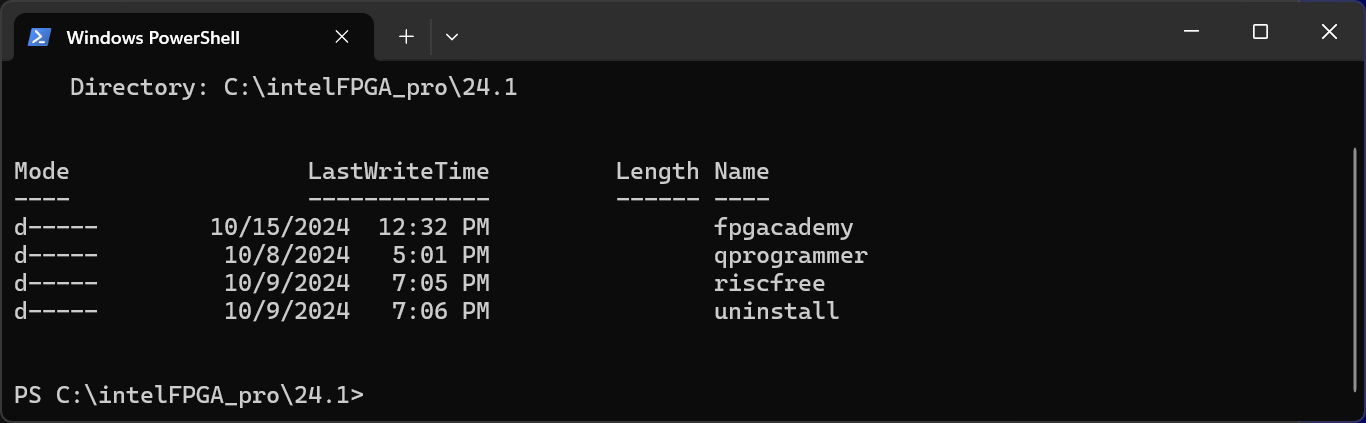
\includegraphics[width=.9\linewidth]{figures/goterdone.png}
        \caption{The final contents of your installation folder.}
        \label{fig:goterdone}
    \end{center}
\end{figure}

\subsection{Installing the Tutorial Design Examples}
\label{sec:egs}

On the {\href{https://www.fpgacademy.org/courses.html} {FPGAcademy.org}} website, this
tutorial is accompanied by {\it Design Files} that are used to illustrate various features
of the {\it GDB} software for developing and debugging Nios~V programs. Download to your 
computer the provided {\it design\_files.zip} file. Then, uncompress this archive into any 
folder of your choice. We will refer to the examples of code and other files in this folder 
throughout the tutorial. Figure~\ref{fig:designfiles} shows the folders included in the
{\it Design Files}, assuming that they have been installed into a folder named
\texttt{GDB\_tutorial}.

\begin{figure}[h]
    \begin{center}
        \includegraphics[width=.9\linewidth]{figures/designfiles.png}
        \caption{The {\it Design Files} folders.}
        \label{fig:designfiles}
    \end{center}
\end{figure}

\section{Setting up the Nios~V Development Environment}
\label{sec:setup}

Once the necessary software and hardware components have been installed onto your computer, 
as discussed in Section~\ref{sec:getthem}, then you can begin working with the {\it GDB}
debugger to develop Nios~V programs. In this tutorial, we use the command-line environment 
provided by the {\it Windows PowerShell}.

\subsection{Using the GNU Make Program}

Open a {\it PowerShell} terminal using a method of your choosing.  Then, navigate to the 
{\it design files} folder called \texttt{C:$\backslash$GDB\_tutorial$\backslash$largest\_s}. 
As illustrated in Figure~\ref{fig:largest1}, this folder contains an example of a 
Nios~V assembly-language program, {\it largest.s}, and a {\it Makefile}. 
~\\
\begin{figure}[h]
    \begin{center}
        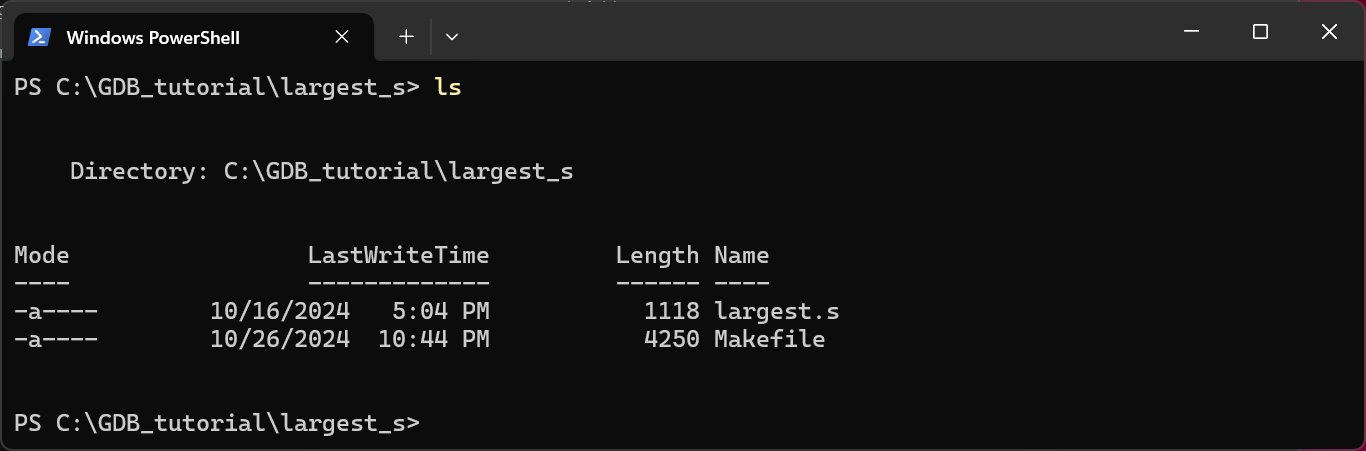
\includegraphics[width=.9\linewidth]{figures/largest1.png}
        \caption{The contents of the largest\_s design files folder.}
        \label{fig:largest1}
    \end{center}
\end{figure}

In this tutorial the tools that we use for developing and debugging Nios~V programs are 
executed via the {\it GNU make} program. A copy of {\it GNU make} is included as part of
the installed software discussed in Section~\ref{sec:getthem}, in the folder:

\texttt{C:$\backslash$intelFPGA\_pro$\backslash$24.1$\backslash$fpgacademy$\backslash$AMP$\backslash$bin}

You should add this folder to your \texttt{Path} {\it Windows Environment Variable}, so
that it is easy to run the {\it make} program.  

\section{Developing and Debugging Nios~V Assembly-Language Programs}
\label{sec:assembly}

In the folder of Figure~\ref{fig:largest1} open the {\it Makefile} in any text editor of your
choice. The first few lines of this file are displayed in Figure~\ref{fig:firstfew}.
Line~1 defines a variable called \texttt{INSTALL} that specifies the folder in which the 
software needed for this tutorial has been installed. The setting given in the figure matches 
the installation folder that we used in Section~\ref{sec:getthem}, as shown in 
Figure~\ref{fig:exe2}. If a different installation folder is used on your computer, then 
change the value of the \texttt{INSTALL} variable accordingly. 

\begin{figure}[h]
    \begin{center}
        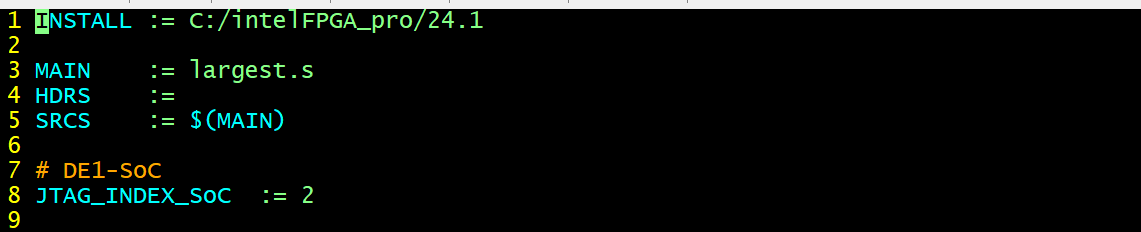
\includegraphics[scale=.5]{figures/firstfew.png}
        \caption{The first few lines of the {\it Makefile}.}
        \label{fig:firstfew}
    \end{center}
\end{figure}

\subsection{Configuring the DE1-SoC Board}

Connect a DE1-SoC board to your computer. The board should be connnected by plugging
a cable that has a {\it Type-A USB} connector into the {\it USB Blaster} port on the board 
and connecting the other end of this cable to any {\it USB} port on your computer. Ensure 
that the DE1-SoC board is properly powered on.

To configure your DE1-SoC board with the desired Nios~V computer system, in the terminal
window of Figure~\ref{fig:largest1} execute the command:

\texttt{make DE1-SoC} 

This command runs the Quartus {\it Programmer} and configures the board with the 
{\it DE1-SoC Computer with Nios~V} system. If the command completes without errors, then you 
can skip ahead to Section~\ref{sec:doit} and begin using GDB with Nios~V. 

If the Quartus {\it Programmer} fails to start, then make sure that you have installed the
required software, and that you have properly set up the \texttt{INSTALL} variable shown
in Figure~\ref{fig:firstfew}. If the Quartus {\it Programmer} runs, but fails to configure 
your DE1-SoC board, then try running the command:

\texttt{make DETECT\_DEVICES}

This command checks which devices are visible on the {\it USB Blaster} cable that is connected to
your computer. Part of the expected output from this command is displayed in
Figure~\ref{fig:detect}. It shows 
two devices being detected: first an {\it SOCVHPS} device, followed by a Cyclone V {\it 5CSE} 
{\it FPGA} device.  If the output produced from your board shows these two devices, but in the 
opposite order, then you have to modify your {\it Makefile}.
Change the variable \texttt{JTAG\_INDEX\_SoC} shown in Line~8 of 
Figure~\ref{fig:firstfew} from the value \texttt{2} to the value \texttt{1}. You should now 
be able to successfully configure your DE1-SoC board by executing the \texttt{make DE1-SoC}
command. Another possible scenario is that you are using a board other 
than the DE1-SoC board. If using the DE10-Lite board, then run the 
command \texttt{make DE10-Lite} to configure your board. If you are using some other board, 
then you will need to read carefully through the {\it Makefile} to determine how its
commands have to be modified to suit your board. 

\begin{figure}[h]
    \begin{center}
        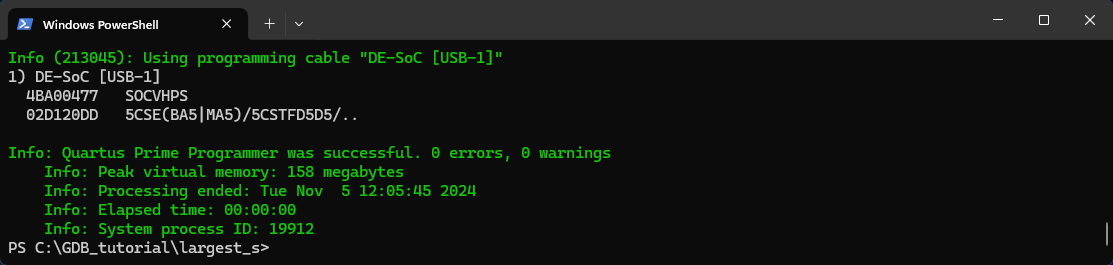
\includegraphics[scale=.55]{figures/detect.png}
        \caption{The output from \texttt{make DETECT\_DEVICES}.}
        \label{fig:detect}
    \end{center}
\end{figure}

\subsection{Using the GDB Server and Client}
\label{sec:doit}

To develop Nios~V programs, you need to use {\bf two} PowerShell terminals: the first one
is used to open the {\it GDB Server}, and the second one is used run the {\it GDB Client}. 
To start the GDB Server, in the terminal window of Figure~\ref{fig:largest1} execute the command:

make \texttt{GDB\_SERVER}

The server will then remain running in this window, as indicated in Figure~\ref{fig:server}. 
Now, open another PowerShell window (you can simply click on the \texttt{+} button near the 
top of Figure~\ref{fig:server} to open a new PoweShell {\it tab}). In this new terminal 
tab navigate again to the same folder as in Figure~\ref{fig:largest1}. 

\begin{figure}[h]
    \begin{center}
        \includegraphics[scale=.55]{figures/server.png}
        \caption{Running the GDB Server.}
        \label{fig:server}
    \end{center}
\end{figure}

The assembly-language program for this part of the tutorial, {\it largest.s}, is shown in 
Figure~\ref{fig:largest_code}. This program searches through a list of integers that is 
stored in memory and finds the largest number in the list. Assemble this program by 
executing the command \texttt{make COMPILE}.
You could also just type \texttt{make}, because \texttt{COMPILE} is the first target in the 
{\it Makefile}. As illustrated in Figure~\ref{fig:make_largest}, this command runs the Nios~V
assembler and linker tools to generate the Nios~V executable file {\it largest.elf}.

\begin{figure}[H]
\lstinputlisting[style=defaultNiosVStyle]{Code/largest.s}
	\caption{A program that finds the largest number in a list.}
	\label{fig:largest_code}
\end{figure}

\begin{figure}[h]
    \begin{center}
        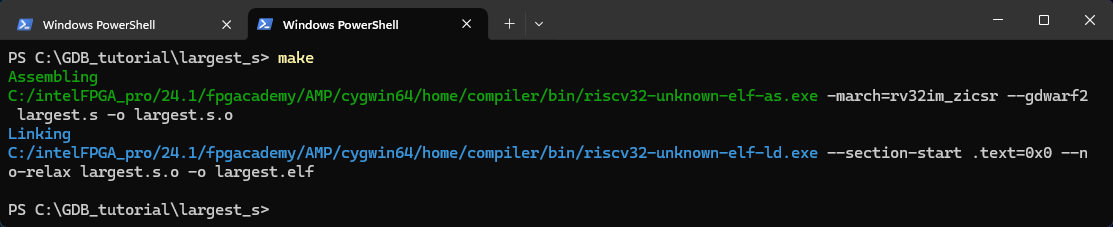
\includegraphics[scale=.55]{figures/make_largest.png}
        \caption{Making the executable file {\it largest.elf}.}
        \label{fig:make_largest}
    \end{center}
\end{figure}

Now you can run the {\it GDB Client} by executing the command:

make \texttt{GDB\_CLIENT}

The GDB Client will connect to your DE1-SoC board, load the executable file {\it largest.elf},
initialize some Nios~V control registers, and set the Nios~V program counter register, {\it pc},
to the start of the program. The output produced by this command is displayed in 
Figure~\ref{fig:gdb_client}.

\begin{figure}[h]
    \begin{center}
        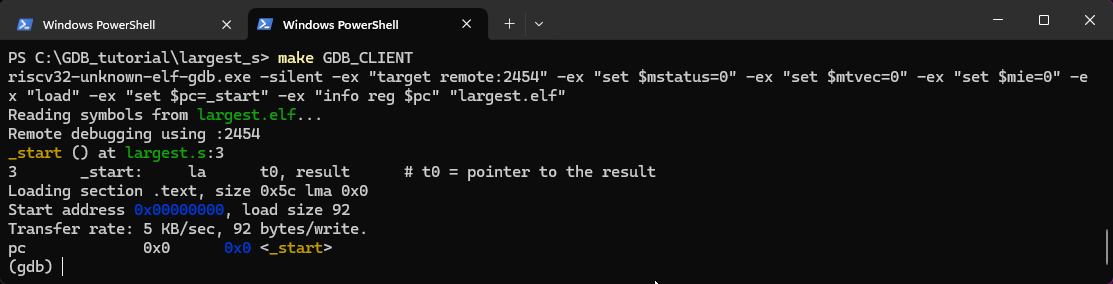
\includegraphics[scale=.6]{figures/gdb_client.png}
        \caption{Starting the GDB Client.}
        \label{fig:gdb_client}
    \end{center}
\end{figure}

In the GDB Client type the \texttt{list} (\texttt{l}) command, as shown in the 
Figure~\ref{fig:gdb1}, to see the loaded program.

\begin{figure}[h]
    \begin{center}
        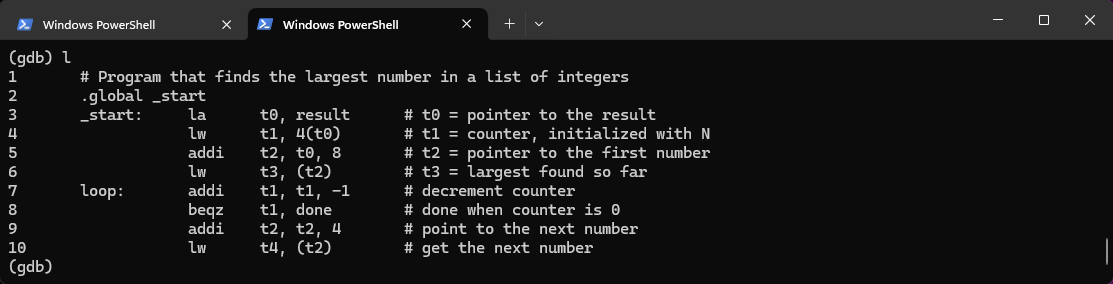
\includegraphics[scale=.6]{figures/gdb1.png}
        \caption{The output of the \texttt{list} command.}
        \label{fig:gdb1}
    \end{center}
\end{figure}

Next, execute the first two instructions in the program by using the 
GDB \texttt{step} (\texttt{s}) command twice. Then, execute the commands 
\texttt{info reg t0} and \texttt{info reg t1} to see that register \texttt{t0} 
holds the address in memory of the \texttt{result} label, which is \texttt{0x38}, and that
register \texttt{t1} has the number of elements in the list, which is \texttt{7} (this value is
specified at the label \texttt{N} in the code Figure~\ref{fig:largest_code}).
The results of these commands are displayed in Figure~\ref{fig:gdb2}.

\begin{figure}[h]
    \begin{center}
        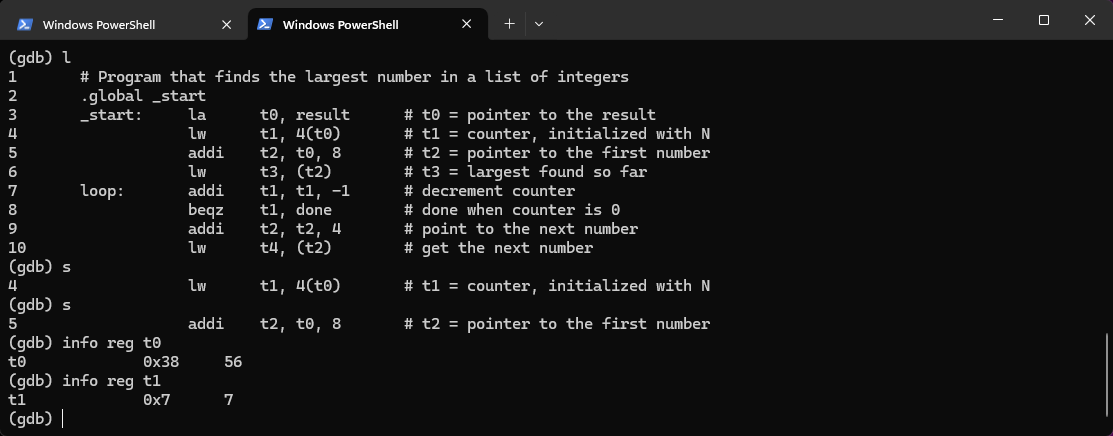
\includegraphics[scale=.6]{figures/gdb2.png}
        \caption{Executing a few GDB commands.}
        \label{fig:gdb2}
    \end{center}
\end{figure}

% Copyright and Trademark

%\newcommand{\datePublished}{Mar 2022}

\newcommand{\versnum}{21.1} %version number quartus/AMP
\newcommand{\quartusname}{Quartus\textsuperscript{\textregistered} Prime}	
\newcommand{\textBar}{For \quartusname{} \versnum{}}
\newcommand{\thisyear}{2022 } %for copyright
\newcommand{\company}{FPGAcademy.org}
\newcommand{\longteamname}{FPGAcademy.org}
\newcommand{\teamname}{FPGAcademy}
\newcommand{\website}{FPGAcademy.org}

\newcommand{\productAcronym}{AMP}
\newcommand{\productNameShort}{Monitor Program}

\newcommand{\productNameMedTM}{Monitor Program}
\newcommand{\productNameMed}{Monitor Program}

%\newcommand{\headerLogoFilePath}[1]{#1/FPGAcademy.png}



%%%%%%%%%%%%%%%%%%%%%%%%%%%%%%%%%%%%%%%%
%%% FPGAcademy Copyright Information %%%
%%%%%%%%%%%%%%%%%%%%%%%%%%%%%%%%%%%%%%%%

%Always put the copyright on a new page (clear page), with some vertical space from top
\clearpage
\vspace{1in}

\noindent

Copyright {\copyright} FPGAcademy.org. All rights reserved. FPGAcademy and the FPGAcademy logo are trademarks of  FPGAcademy.org.  This document is being provided on an ``as-is'' basis and as an accommodation and therefore all warranties, representations or guarantees of any kind (whether express, implied or statutory) including, without limitation, warranties of merchantability, non-infringement, or fitness for a particular purpose, are specifically disclaimed.

%FPGAcademy assumes no responsibility or liability arising out of the application or use of any information,  product,  or  service  described  herein  except  as  expressly  agreed  to  in  writing  by  FPGAcademy.



**Other names and brands may be claimed as the property of others.




\end{document}
